%\documentclass{article}
%\usepackage{graphicx,subfigure,lscape}
%\begin{document}

\begin{landscape}
\begin{figure}[h]
  \centering
  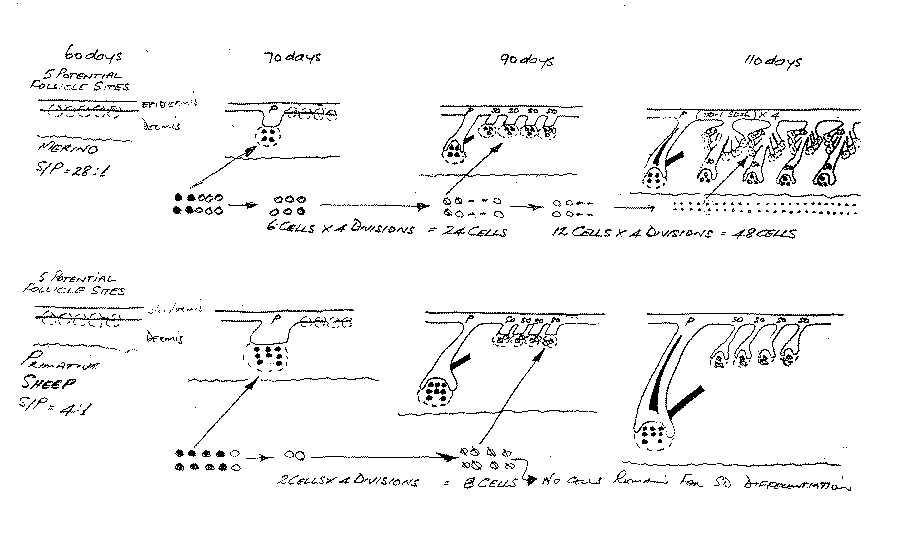
\includegraphics[width=1.9\textwidth,trim = 20 0 0 80]{images/fig16.png}
  \caption{  A quantitative illustration of predictions which can be made with
      the Moore hypothesis regarding the role of primary follicle size
      in determining comparative development of Merino and primitive
      foetal skin over the period 60-110 days of gestation.  Note that
      this presentation is diagrammatic - relative sizes and shapes of
      follicles are not able to accurately represent reality, and cell
      numbers and division rates should not be taken to be absolute.
      For a complete explanation see text.}
  \label{fig:16}
\end{figure}
\end{landscape}

%\end{document}
